\documentclass[12pt,a4paper]{report}

% ----------------------------------------------------
% PACKAGES
% ----------------------------------------------------
\usepackage{color}
\usepackage{fancyhdr}
\usepackage{setspace}
\usepackage{titlesec}
\usepackage{geometry}
\usepackage{graphicx}
\usepackage{enumitem}
\usepackage{ragged2e}
\usepackage{lipsum}
\usepackage{tocloft}
\usepackage{tikz}
\usetikzlibrary{shapes.geometric, shapes.multipart, arrows.meta, positioning, fit, backgrounds}
\usepackage{textcomp}

\geometry{
    top=1.25in,
    bottom=1.25in,
    left=1in,
    right=1in
}

% ----------------------------------------------------
% HEADER & FOOTER SETUP
% ----------------------------------------------------
\pagestyle{fancy}
\fancyhf{}
\fancyhead[L]{\leftmark}
\renewcommand{\headrulewidth}{0.4pt}
\fancyfoot[L]{\textbf{Dnyanshree Institute of Engineering and Technology, Satara \\ Department of Computer Science and Engineering}}
\fancyfoot[R]{\thepage}
\renewcommand{\footrulewidth}{0.4pt}
\setlength{\footskip}{25pt}

\fancypagestyle{plain}{
    \fancyhf{}
    \fancyhead[L]{\leftmark}
    \renewcommand{\headrulewidth}{0.4pt}
    \fancyfoot[L]{\textbf{Dnyanshree Institute of Engineering and Technology, Satara \\ Department of Computer Science and Engineering}}
    \fancyfoot[R]{\thepage}
    \renewcommand{\footrulewidth}{0.4pt}
}

% ----------------------------------------------------
% DOCUMENT BEGINS
\begin{document}

% ============================================================
% ======================== INITIAL PAGES =====================
% ============================================================

% ============================================================
% ------------------------ COVER PAGE -------------------------
% ============================================================
\thispagestyle{empty}
\begin{center}

{\large \textbf{A}}\\[4pt]
{\large \textbf{MINI PROJECT II}}\\[4pt]
{\large \textbf{REPORT ON}}\\[4pt]

{\Large \bfseries \color{blue}
Handwritten Digit Recognition Model}\\[20pt]

{\normalsize Submitted in Partial Fulfillment of Requirement for the award of\\
degree of}\\[14pt]

{\large \textbf{BACHELOR OF TECHNOLOGY}}\\[4pt]
{\large \bfseries \color{magenta} COMPUTER SCIENCE AND ENGINEERING}\\[14pt]

{\normalsize DR. BABASAHEB AMBEDKAR TECHNOLOGICAL\\
UNIVERSITY, LONERE}\\[20pt]

{\normalsize Submitted By}\\[10pt]

\begin{tabular}{l c}
\textbf{Name of Students} & \textbf{PRN No.} \\
Aarya Dilip Jadhav         & 23067971242031 \\
Onkar Yashawantrao Ghadage         & 23067971242032 \\
Vishwajeet Janardan Kumbhar         & 23067971242065 \\
Zeenat Juber Shaikh         & 23067971242078 \\
\end{tabular}\\[25pt]

{\normalsize Under the guidance of}\\[4pt]
{\normalsize \textbf{Prof. M. M. Ghorpade}}\\[16pt]

\includegraphics[width=3cm]{image1.png}\\[18pt]

{\small RAOSAHEB WANGDE MASTER CHARITABLE TRUST'S}\\[6pt]

{\Large \bfseries \color{red}
Dnyanshree Institute Of Engineering and \\
Technology}\\[6pt]

{\normalsize Sajjangad Road, Satara, Maharashtra State, 415 013, (India)}\\[20pt]

{\large \textbf{Academic Year 2025-26}}

\end{center}
\newpage

% ============================================================
% ----------------------- CERTIFICATE PAGE --------------------
% ============================================================
\thispagestyle{empty}
\begin{center}
{\Large \bfseries \color{red} Certificate}\\[20pt]
\end{center}

\begin{justify}
{\normalsize
This is to certify that the project entitled,
\textbf{"Handwritten Digit Recognition model"} is submitted by
}
\end{justify}

\begin{center}
\begin{tabular}{l c c}
\textbf{Name of Students} & \textbf{PRN No.} & \textbf{Exam Seat No.} \\
Aarya Dilip Jadhav         & 23067971242031 & 23213015 \\
Onkar Yashawantrao Ghadage         & 23067971242032 & 23213016 \\
Vishwajeet Janardan Kumbhar         & 23067971242065 & 23213004 \\
Zeenat Juber Shaikh         & 23067971242078 & 23213008 \\
\end{tabular}
\end{center}

\begin{justify}
{\normalsize
It is bonafide work carried out by these students under the guidance of
Prof. M. M. Ghorpade.
It has been accepted and approved for the partial fulfilment of the requirement of
Dr. Babasaheb Ambedkar Technological University, Lonere, for the award of the
degree of Bachelor of Technology (Computer Science and Engineering).
This work and project report has not been earlier submitted to any other Institute
or University for the award of any degree or diploma.
}
\end{justify}

\begin{table*}[h!]
\centering
\begin{tabular}{p{5cm} p{6cm} p{7cm}} \\ \\ \\ \\ \\ \\ \\ \\
\textbf{Signature:} & \textbf{Signature:} & \textbf{Signature:} \\
\textbf{Prof. M. M. Ghorpade}      & \textbf{Prof. P. M. Pondkule}      & \textbf{Dr. A. D. Jadhav}      \\
\textbf{[Guide]}    & \textbf{[Head of Department]} & \textbf{[Principal]} \\
\end{tabular}
\end{table*}

\begin{flushleft}
\textbf{Signature:}\\[4pt]
\textbf{Name:}\\
\textbf{[External Examiner]}\\[20pt]

\textbf{Place:} Satara\\
\textbf{Date:}
\end{flushleft}
\newpage

% ============================================================
% -------------------- ACKNOWLEDGMENT PAGE --------------------
% ============================================================
\thispagestyle{empty}

\begin{center}
{\Large \bfseries \color{red} Acknowledgments}
\end{center}

\vspace{20pt}

\begin{justify}
{\normalsize
The satisfaction and euphoria that accompany the successful completion of any
task would be incomplete without the mention of people who made it possible.
So, we acknowledged all those whose guidance and encouragement served as a
beacon of light and crowned our efforts with success.\\ \\
We have immense pleasure in expressing thanks to the Principal
\textbf{Dr. A. D. Jadhav}, for providing all the facilities for the successful
completion of the project.\\ \\
Our profound sense of gratitude is due to our Head of the Department
\textbf{Prof. P. M. Pondkule}, for constant encouragement, valuable guidance and
also for the inspiration to pursue the project.\\ \\
We also thanks to \textbf{Prof. M. M. Ghorpade} Project Coordinator, for their guidance
and for being a constant source of support and guided us in this Endeavour.\\
Last but not the least we are thankful to all faculty members and lab instructors
without whose support at various stages, this project would not have materialized.\\ \\
}
\end{justify}

\vspace{40pt}

\begin{flushright}
{\normalsize
\textbf{"Thanking You"\\[6pt]
Aarya Dilip Jadhav\\
Onkar Yashawantrao Ghadage\\
Vishwajeet Janardan Kumbhar\\
Zeenat Juber Shaikh\\
}}
\end{flushright}

\vspace{40pt}

\begin{flushleft}
{\normalsize
\textbf{Date:}\\
\textbf{Place:} Satara
}
\end{flushleft}

\newpage

% ============================================================
% ========================== INDEX ===========================
% ============================================================

% ============================================================
% LIST OF FIGURES
% ============================================================
\section*{List of Figures \\}
\begin{flushleft}
\begin{tabular}{p{0.7cm} p{13.5cm} p{1.5cm}}

1  & System Architecture                                                   \dotfill & 14  \\[0.50cm]
2  & Data Flow Diagram Level 0                                             \dotfill & 19 \\[0.50cm]
3  & Data Flow Diagram Level 1                                             \dotfill & 20 \\[0.50cm]
4  & Use Case Diagram                                                      \dotfill & 21 \\[0.50cm]
5  & Activity Diagram                                                      \dotfill & 22 \\[0.50cm]
6  & Component Diagram                                                     \dotfill & 23 \\[0.50cm]
7  & Sequence Diagram                                                      \dotfill & 24 \\[0.50cm]
8  & Draw Tab -- User draws a digit on the canvas                          \dotfill & 28 \\[0.50cm]
9  & Prediction Result -- Low Confidence Score                             \dotfill & 29 \\[0.50cm]
10 & Prediction Result -- High Confidence Score (100\%)                    \dotfill & 30 \\[0.50cm]
11 & Upload Tab -- User uploads an image of a handwritten digit            \dotfill & 31 \\[0.50cm]

\end{tabular}
\end{flushleft}

\newpage

% ============================================================
% ABSTRACT
% ============================================================
\begin{center}
{\Large \bfseries Abstract}\\[30pt]
\end{center}

The Handwritten Digit Recognizer is a deep learning based web application that automatically identifies handwritten digits from 0 to 9. The system uses a Convolutional Neural Network (CNN) trained on the MNIST dataset, which contains 70,000 grayscale images of handwritten digits. Users can interact with the application through two modes: drawing a digit directly on an interactive canvas or uploading an image file. The input is preprocessed through grayscale conversion, background inversion, bounding box cropping, and resizing before being passed to the CNN model. The model achieves approximately 99\% accuracy on the MNIST test set and returns an instant prediction along with a confidence score and a per-digit probability bar chart. The application is deployed using the Streamlit framework and runs in any modern web browser without requiring any installation.\\ \\
\textbf{Keywords:} Handwritten digit recognition, Convolutional Neural Network, MNIST, deep learning, image classification, Streamlit, TensorFlow, Keras, image preprocessing.

\newpage

% ============================================================
% TABLE OF CONTENTS
% ============================================================
\section*{Contents \\}

\noindent
1.\quad \textbf{Introduction} \hfill 8\\[20pt]

\noindent
2.\quad \textbf{Literature Review} \hfill 9\\[12pt]
\hspace*{1cm}2.1\quad \textbf{Technology Description} \dotfill 10\\[12pt]
\hspace*{1cm}2.2\quad \textbf{Platforms} \dotfill 12\\[20pt]

\noindent
3.\quad \textbf{Design, Development and Drawing} \hfill 13\\[12pt]
\hspace*{1cm}3.1\quad \textbf{Proposed Work} \dotfill 13\\[12pt]
\hspace*{2cm}3.1.1\quad Problem Statement \dotfill 13\\[12pt]
\hspace*{2cm}3.1.2\quad Objectives \dotfill 13\\[12pt]
\hspace*{2cm}3.1.3\quad Title \dotfill 13\\[12pt]
\hspace*{1cm}3.2\quad \textbf{Design} \dotfill 14\\[12pt]
\hspace*{2cm}3.2.1\quad System Architecture \dotfill 14\\[12pt]
\hspace*{1cm}3.3\quad \textbf{Development} \dotfill 16\\[12pt]
\hspace*{2cm}3.3.1\quad CNN Model Architecture \dotfill 16\\[12pt]
\hspace*{2cm}3.3.2\quad Image Preprocessing \dotfill 16\\[12pt]
\hspace*{2cm}3.3.3\quad Software Requirements Specifications \dotfill 17\\[12pt]
\hspace*{2cm}3.3.4\quad Hardware Requirements Specifications \dotfill 17\\[12pt]
\hspace*{1cm}3.4\quad \textbf{Drawing} \dotfill 19\\[12pt]
\hspace*{2cm}3.4.1\quad Data Flow Diagram Level 0 \dotfill 19\\[12pt]
\hspace*{2cm}3.4.2\quad Data Flow Diagram Level 1 \dotfill 20\\[12pt]
\hspace*{1cm}3.5\quad \textbf{UML Diagram} \dotfill 21\\[12pt]
\hspace*{2cm}3.5.1\quad Use Case Diagram \dotfill 21\\[12pt]
\hspace*{2cm}3.5.2\quad Activity Diagram \dotfill 22\\[12pt]
\hspace*{2cm}3.5.3\quad Component Diagram \dotfill 23\\[12pt]
\hspace*{2cm}3.5.4\quad Sequence Diagram \dotfill 24\\[20pt]

\noindent
4.\quad \textbf{Experimentation, Results and Discussion} \hfill 25\\[12pt]
\hspace*{1cm}4.1\quad \textbf{Experimentation} \dotfill 25\\[12pt]
\hspace*{2cm}4.1.1\quad Model Training Experiment \dotfill 25\\[12pt]
\hspace*{2cm}4.1.2\quad Testing with Drawn Digits \dotfill 26\\[12pt]
\hspace*{2cm}4.1.3\quad Testing with Uploaded Images \dotfill 26\\[12pt]
\hspace*{2cm}4.1.4\quad Testing with Edge Cases \dotfill 26\\[12pt]
\hspace*{1cm}4.2\quad \textbf{Results} \dotfill 27\\[12pt]
\hspace*{2cm}4.2.1\quad Model Performance \dotfill 27\\[12pt]
\hspace*{2cm}4.2.2\quad Application Performance \dotfill 27\\[12pt]
\hspace*{2cm}4.2.3\quad Screenshots \dotfill 28\\[12pt]
\hspace*{1cm}4.3\quad \textbf{Discussion} \dotfill 32\\[20pt]

\noindent
5.\quad \textbf{Conclusion and Future Scope} \hfill 33\\[12pt]
\hspace*{1cm}5.1\quad \textbf{Conclusion} \dotfill 33\\[12pt]
\hspace*{1cm}5.2\quad \textbf{Future Scope} \dotfill 33\\[12pt]
\hspace*{1cm}\textbf{References} \dotfill 34\\[12pt]

\newpage

% ============================================================
% ========================== MAIN ============================
% ============================================================

%-------------------------
\chapter{Introduction}

Handwritten digit recognition is one of the most well-studied problems in the field of machine learning and computer vision. The ability of a computer to automatically identify digits written by hand has a wide range of real-world applications, including postal code reading, bank cheque processing, form digitization, and educational tools. Despite the simplicity of the task for humans, teaching a machine to reliably recognize handwritten digits requires careful design of the learning model and training process.\\ \\
The Handwritten Digit Recognizer is an interactive web application that allows users to either draw a digit on a canvas or upload an image of a handwritten digit, and receive an instant prediction along with a confidence score. The system is powered by a Convolutional Neural Network (CNN) trained on the MNIST dataset, which contains 70,000 grayscale images of handwritten digits from 0 to 9. The trained model is deployed using Streamlit, making it accessible through any modern web browser without requiring any installation. This project demonstrates the practical application of deep learning in building intelligent systems. It bridges the gap between theoretical machine learning concepts and real-world deployment by combining model training, preprocessing, and a user-friendly interface into a single working application. The goal is to provide an accurate, fast, and easy-to-use tool that showcases the power of CNNs for image classification tasks.

%---------------------------------
\chapter{Literature Review}

\begin{table}[h!]
\centering
\caption{Literature Review on Handwritten Digit Recognition}
\begin{tabular}{|p{1cm}|p{3cm}|p{4cm}|p{3cm}|p{4cm}|}
\hline
\textbf{Sr. No.} & \textbf{Paper Title} & \textbf{Author} & \textbf{Year of Publication} & \textbf{Details of work carried out} \\
\hline

1 & Gradient-Based Learning Applied to Document Recognition &
Yann LeCun, Léon Bottou, Yoshua Bengio \& Patrick Haffner & 1998 & Introduced the LeNet-5 CNN architecture for handwritten digit recognition on MNIST, achieving over 99\% accuracy and establishing the foundation for modern deep learning in image classification. \\
\hline

2 & Dropout: A Simple Way to Prevent Neural Networks from Overfitting &
Nitish Srivastava, Geoffrey Hinton, Alex Krizhevsky, Ilya Sutskever \& Ruslan Salakhutdinov & 2014 & Proposed the dropout regularization technique, which randomly disables neurons during training to prevent overfitting, significantly improving generalization on tasks like MNIST digit classification. \\
\hline

\end{tabular}
\end{table}

\begin{table}[h!]
\centering
\caption{Literature Review on Handwritten Digit Recognition (Continued)}
\begin{tabular}{|p{1cm}|p{3cm}|p{4cm}|p{3cm}|p{4cm}|}
\hline
\textbf{Sr. No.} & \textbf{Paper Title} & \textbf{Author} & \textbf{Year of Publication} & \textbf{Details of work carried out} \\
\hline

3 & ImageNet Classification with Deep Convolutional Neural Networks &
Alex Krizhevsky, Ilya Sutskever \& Geoffrey Hinton & 2012 & Demonstrated the power of deep CNNs with ReLU activations and max-pooling for image classification, influencing the design of digit recognition models that use similar architectural patterns. \\
\hline

4 & An Introduction to Convolutional Neural Networks &
Keiron O'Shea \& Ryan Nash & 2015 & Provided a detailed overview of CNN components including convolutional layers, pooling layers, and fully connected layers, directly applicable to understanding the architecture used in handwritten digit recognition. \\
\hline

\end{tabular}
\end{table}

\newpage
\section{Technology Description}
The Handwritten Digit Recognizer is developed using Python-based machine learning and web technologies. The project focuses on combining a trained deep learning model with an interactive user interface, making it accessible and easy to use.

\subsection*{1. Python}
Python is the primary programming language used throughout the project. It is used for data preprocessing, model training, and building the web application. Python's rich ecosystem of libraries makes it ideal for machine learning projects.

\subsection*{2. TensorFlow and Keras}
TensorFlow is an open-source deep learning framework used to build and train the CNN model. Keras, which is integrated into TensorFlow, provides a high-level API that simplifies the process of defining layers, compiling the model, and running training. The trained model is saved in the HDF5 format (\texttt{mnist\_cnn.h5}) for later use.

\subsection*{3. MNIST Dataset}
The MNIST (Modified National Institute of Standards and Technology) dataset is the standard benchmark dataset for handwritten digit recognition. It contains 60,000 training images and 10,000 test images of handwritten digits from 0 to 9, each of size 28×28 pixels in grayscale.

\subsection*{4. Streamlit}
Streamlit is a Python framework used to build the interactive web application. It allows the model to be deployed as a browser-based tool without requiring any web development knowledge. Streamlit handles the UI components, file uploads, and real-time predictions.

\subsection*{5. streamlit-drawable-canvas}
This Streamlit component provides a drawable canvas widget that allows users to draw digits directly in the browser using their mouse or touchscreen. The drawn image is then passed to the model for prediction.

\subsection*{6. NumPy and Pillow}
NumPy is used for numerical operations and array manipulation during image preprocessing. Pillow (PIL) is used for image loading, conversion, resizing, and inversion to prepare uploaded images for model input.

\newpage
\section{Platforms}
The Handwritten Digit Recognizer is a Python-based web application that runs locally on any machine with Python installed. The following platforms and tools were used during development and deployment.

\subsection*{1. Web Browser}
The Streamlit application runs in any modern web browser such as Google Chrome, Microsoft Edge, or Mozilla Firefox. Users access the application through a local URL generated when the app is launched, requiring no installation on the user's side.

\subsection*{2. Jupyter Notebook}
Jupyter Notebook was used for the model training phase. The notebook (\texttt{mnist\_training.ipynb}) contains all steps from data loading and preprocessing to model building, training, evaluation, and saving.

\subsection*{3. Git and GitHub}
Git was used for version control during development. The project is hosted on GitHub for storage, collaboration, and easy sharing with evaluators.

\subsection*{4. Visual Studio Code}
VS Code was used as the primary code editor for writing and editing the Streamlit application code. Its Python extension, integrated terminal, and debugging tools made development efficient.

\subsection*{5. Python Virtual Environment}
A Python virtual environment (\texttt{venv}) was used to isolate project dependencies. All required packages are listed in \texttt{requirements.txt}, allowing the project to be reproduced on any machine.

\chapter{Design, Development and Drawing}
\section{Proposed Work}
\subsection{Problem Statement}
Manually reading and digitizing handwritten digits is time-consuming and error-prone, so an automated system is needed that can accurately recognize handwritten digits from drawn or uploaded images using deep learning techniques.

\subsection{Objectives}
1. To develop a handwritten digit recognition system using CNN. \\ \\
2. To allow users to draw or upload handwritten digit images. \\ \\
3. To preprocess images for accurate digit prediction. \\ \\
4. To predict digits from 0 to 9 with confidence scores. \\ \\
5. To create a simple and user-friendly web interface using Streamlit. \\ \\

\subsection{Title} Handwritten Digit Recognizer \\ \\

\section{Design}
\subsection{System Architecture}
The Handwritten Digit Recognizer is built as a layered system where each layer has a specific responsibility. The architecture consists of five layers stacked from the user down to the final output, with data flowing downward through each layer and the result returned to the user at the end.\\

\begin{figure}[h!]
\centering
\includegraphics[width=0.35\textwidth]{System_Architecture.png}
\caption{System Architecture}
\label{fig:myimage}
\end{figure}

\subsubsection{User Layer}
The topmost layer represents the end user who interacts with the system through a web browser. The user can either draw a digit directly on the canvas using a mouse or touchscreen, or upload an existing image file of a handwritten digit. This layer is the entry point of the entire system.

\subsubsection{Streamlit Web Interface Layer}
This layer is the front-end of the application built using the Streamlit framework. It renders the drawable canvas, the file upload widget, the Predict button, and all output elements. It acts as the bridge between the user and the internal processing modules, capturing user input and passing it to the preprocessing layer.

\subsubsection{Image Preprocessing Layer}
This layer is responsible for converting any input image into the exact format the CNN model expects. It performs grayscale conversion, background auto-inversion so the digit is always white on black, bounding box cropping to remove empty space, resizing to 20×20 with padding to 28×28, and normalization of pixel values to the range 0--1. Without this layer, the model would produce unreliable results on real-world inputs.

\subsubsection{CNN Model Layer}
This is the core intelligence of the system. The pre-trained Convolutional Neural Network stored in \texttt{mnist\_cnn.h5} receives the 28×28 normalized array and performs a forward pass through its layers -- two convolutional blocks for feature extraction, a dropout layer for regularization, and dense layers for classification. It outputs a probability array of 10 values, one for each digit class from 0 to 9.

\subsubsection{Prediction Output Layer}
The bottommost layer takes the probability array from the CNN and presents the results to the user. It identifies the digit with the highest probability as the predicted digit, calculates the confidence percentage, and renders a bar chart showing the probability distribution across all 10 digit classes. Feedback messages are also shown based on the confidence level.

\newpage
\section{Development}
\subsection{CNN Model Architecture}
The model is a Sequential CNN with the following layers:

\begin{enumerate}
    \item \textbf{Conv2D (32 filters, 3×3, ReLU)} -- Detects low-level features such as edges and curves in the 28×28 input image.
    \item \textbf{MaxPooling2D (2×2)} -- Reduces spatial dimensions by half, retaining the most prominent features.
    \item \textbf{Conv2D (64 filters, 3×3, ReLU)} -- Learns more complex and abstract features from the downsampled feature maps.
    \item \textbf{MaxPooling2D (2×2)} -- Further reduces spatial dimensions.
    \item \textbf{Flatten} -- Converts the 2D feature maps into a 1D vector for the dense layers.
    \item \textbf{Dropout (0.5)} -- Randomly disables 50\% of neurons during training to prevent overfitting.
    \item \textbf{Dense (128 neurons, ReLU)} -- Performs high-level reasoning on the extracted features.
    \item \textbf{Dense (10 neurons, Softmax)} -- Outputs a probability for each of the 10 digit classes (0--9).
\end{enumerate}

The model is compiled with the Adam optimizer, sparse categorical cross-entropy loss, and accuracy as the evaluation metric. It is trained for 10 epochs with a batch size of 64 and a 10\% validation split.

\subsection{Image Preprocessing}
A key part of the application is the preprocessing function that converts any input image into the 28×28 grayscale format the model expects:
\begin{enumerate}
    \item Convert the image to grayscale.
    \item Auto-detect background: if the image is mostly light (e.g., a photo on white paper), invert it so the digit is white on a black background, matching the MNIST format.
    \item Crop to the bounding box of the digit to remove excess whitespace.
    \item Resize to 20×20 while preserving aspect ratio, then pad to 28×28 with a black border.
    \item Normalize pixel values to the range 0--1 and reshape to (1, 28, 28, 1).
\end{enumerate}

\subsection{Software Requirements Specifications}
\begin{enumerate}
    \item \textbf{Software Compatibility}
    \begin{itemize}
        \item Windows 10 / 11
        \item Linux distributions
        \item macOS
        \item Modern web browsers (Chrome, Edge, Firefox, Safari)
    \end{itemize}
    \item \textbf{Programming Languages}
    \begin{itemize}
        \item Python 3.9 or higher
    \end{itemize}
    \item \textbf{Development Tools}
    \begin{itemize}
        \item Visual Studio Code
        \item Jupyter Notebook / JupyterLab
        \item Git
        \item GitHub
        \item Python Virtual Environment (venv)
    \end{itemize}
    \item \textbf{Libraries and Frameworks}
    \begin{itemize}
        \item TensorFlow 2.x / Keras
        \item Streamlit
        \item streamlit-drawable-canvas
        \item NumPy
        \item Pillow (PIL)
        \item Matplotlib
    \end{itemize}
\end{enumerate}

\subsection{Hardware Requirements Specifications}
\begin{enumerate}
    \item \textbf{Client-Side Requirements}
    \begin{itemize}
        \item Minimum Requirements
        \begin{itemize}
            \item[] -- Processor: Dual-core processor (Intel/AMD/ARM)
            \item[] -- RAM: 4 GB or higher
            \item[] -- Storage: At least 500 MB free space for model and dependencies
            \item[] -- Display: 720p resolution or higher
        \end{itemize}
        \item Recommended Requirements
        \begin{itemize}
            \item[] -- Processor: Intel i5 or equivalent
            \item[] -- RAM: 8 GB or higher
            \item[] -- Display: Full HD for better UI experience
            \item[] -- Modern Web Browser: Chrome, Edge, or Firefox
        \end{itemize}
    \end{itemize}
    \item \textbf{Development Environment}
    \begin{itemize}
        \item Development Machine Requirements
        \begin{itemize}
            \item[] -- Processor: Intel i5 / Ryzen 5 or higher (GPU optional but beneficial for training)
            \item[] -- RAM: 8 GB or more
            \item[] -- Storage: At least 3 GB free space (for Python, TensorFlow, project files)
            \item[] -- Operating System: Windows 10/11, Linux, or macOS
        \end{itemize}
        \item Tools Used in Development
        \begin{itemize}
            \item[] -- Visual Studio Code
            \item[] -- Jupyter Notebook
            \item[] -- Git and GitHub
            \item[] -- Multiple web browsers for testing
        \end{itemize}
    \end{itemize}
\end{enumerate}

\newpage
\section{Drawing}
\subsection{Data Flow Diagram Level 0}
DFD Level 0 shows the overall working of the Handwritten Digit Recognizer as a single process. The only external entity is the User, who provides a handwritten digit either by drawing on the canvas or uploading an image. The system processes this input and returns a prediction indicating the recognized digit along with a confidence score. This diagram represents the basic flow of data between the user and the system without showing any internal steps.
\begin{figure}[h!]
\centering
\includegraphics[width=0.85\textwidth]{DFD0.png}
\caption{Data Flow Diagram Level 0}
\label{fig:dfd0}
\end{figure}

\newpage
\subsection{Data Flow Diagram Level 1}
DFD Level 1 explains the internal working of the Handwritten Digit Recognizer. The user provides a digit image, which is first received by the Input Handling process. The image is then passed to the Preprocessing process, where it is converted to the correct format. Finally, the Model Inference process runs the CNN and the Result Display process sends the predicted digit and confidence back to the user.

\begin{figure}[h!]
\centering
\includegraphics[width=0.8\textwidth]{DFD1.png}
\caption{Data Flow Diagram Level 1}
\label{fig:dfd1}
\end{figure}

\newpage
\section{UML Diagram}
\subsection{Use Case Diagram}
The Use Case Diagram shows the interaction between the user and the Handwritten Digit Recognizer system. The user can draw a digit on the canvas or upload an image file. After providing input, the user can trigger a prediction and view the result, which includes the predicted digit, confidence percentage, and a per-digit probability bar chart. The user can also clear the canvas and draw again or upload a different image.

\begin{figure}[h!]
\centering
\includegraphics[width=0.7\textwidth]{usecase (1).png}
\caption{Use Case Diagram}
\label{fig:usecase}
\end{figure}

\newpage
\subsection{Activity Diagram}
The Activity Diagram shows the flow of actions in the Handwritten Digit Recognizer. The process starts when the user opens the application in a browser. The user selects either the Draw tab or the Upload tab. In the Draw tab, the user draws a digit and clicks Predict. In the Upload tab, the user selects an image file and clicks Predict. In both cases, the system preprocesses the input, runs the CNN model, and displays the prediction result. The user can then repeat the process with a new digit.

\begin{figure}[h!]
\centering
\includegraphics[width=0.5\textwidth]{activiity.png}
\caption{Activity Diagram}
\label{fig:activity}
\end{figure}

\newpage
\subsection{Component Diagram}
The Component Diagram represents the main structural parts of the Handwritten Digit Recognizer system and how they interact with each other. The system is divided into four major components: the User Interface component built with Streamlit, the Preprocessing component that handles image conversion, the CNN Model component that performs digit classification, and the MNIST Training component that was used offline to produce the saved model. The UI component communicates with the Preprocessing component, which in turn feeds data to the CNN Model component. The saved model file (\texttt{mnist\_cnn.h5}) acts as the bridge between the offline training phase and the live inference phase.\\

\begin{figure}[h!]
\centering
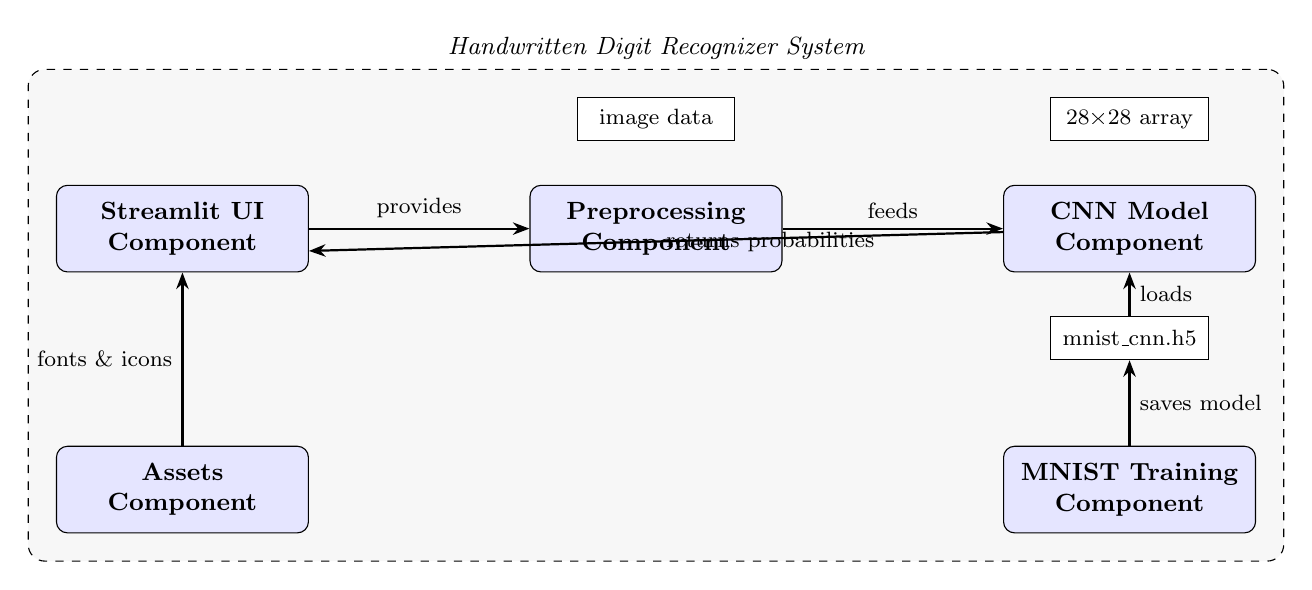
\begin{tikzpicture}[
    comp/.style={
        draw, rectangle, rounded corners=4pt,
        minimum width=3.2cm, minimum height=1.1cm,
        fill=blue!10, font=\small\bfseries, align=center
    },
    iface/.style={
        draw, rectangle,
        minimum width=2cm, minimum height=0.55cm,
        fill=white, font=\footnotesize, align=center
    },
    pkg/.style={
        draw, dashed, rounded corners=6pt,
        inner sep=10pt, fill=gray!6
    },
    arr/.style={-{Stealth[length=6pt]}, thick},
    node distance=1.4cm and 2.6cm
]

\node[comp] (ui)      {Streamlit UI\\Component};
\node[comp, right=2.8cm of ui]  (pre)  {Preprocessing\\Component};
\node[comp, right=2.8cm of pre] (cnn)  {CNN Model\\Component};
\node[comp, below=2.2cm of cnn] (train){MNIST Training\\Component};
\node[comp, below=2.2cm of ui]  (asset){Assets\\Component};

\node[iface, above=0.55cm of pre] (i1) {image data};
\node[iface, above=0.55cm of cnn] (i2) {28×28 array};
\node[iface, below=0.55cm of cnn] (i3) {mnist\_cnn.h5};

\draw[arr] (ui)  -- node[above, font=\footnotesize]{provides} (pre);
\draw[arr] (pre) -- node[above, font=\footnotesize]{feeds}    (cnn);
\draw[arr] (cnn) -- node[right, font=\footnotesize]{returns probabilities} (ui.-10) [bend right=40];
\draw[arr] (train) -- node[right, font=\footnotesize]{saves model} (i3);
\draw[arr] (i3)    -- node[right, font=\footnotesize]{loads}       (cnn);
\draw[arr] (asset) -- node[left,  font=\footnotesize]{fonts \& icons} (ui);

\begin{scope}[on background layer]
    \node[pkg, fit=(ui)(pre)(cnn)(asset)(train)(i1)(i2)(i3),
          label={[font=\small\itshape]above:Handwritten Digit Recognizer System}] {};
\end{scope}

\end{tikzpicture}
\caption{Component Diagram}
\label{fig:component}
\end{figure}

\newpage
\subsection{Sequence Diagram}
The Sequence Diagram shows the time-ordered interaction between the User, the Streamlit UI, the Preprocessing module, and the CNN Model during a single prediction request. The user either draws a digit or uploads an image. The UI captures the input and passes it to the Preprocessing module, which converts it to the 28×28 normalized format. The preprocessed array is then sent to the CNN Model, which returns a probability array of 10 values. The UI reads the highest probability, formats the result, and displays the predicted digit along with the confidence score and bar chart to the user.\\

\begin{figure}[h!]
\centering
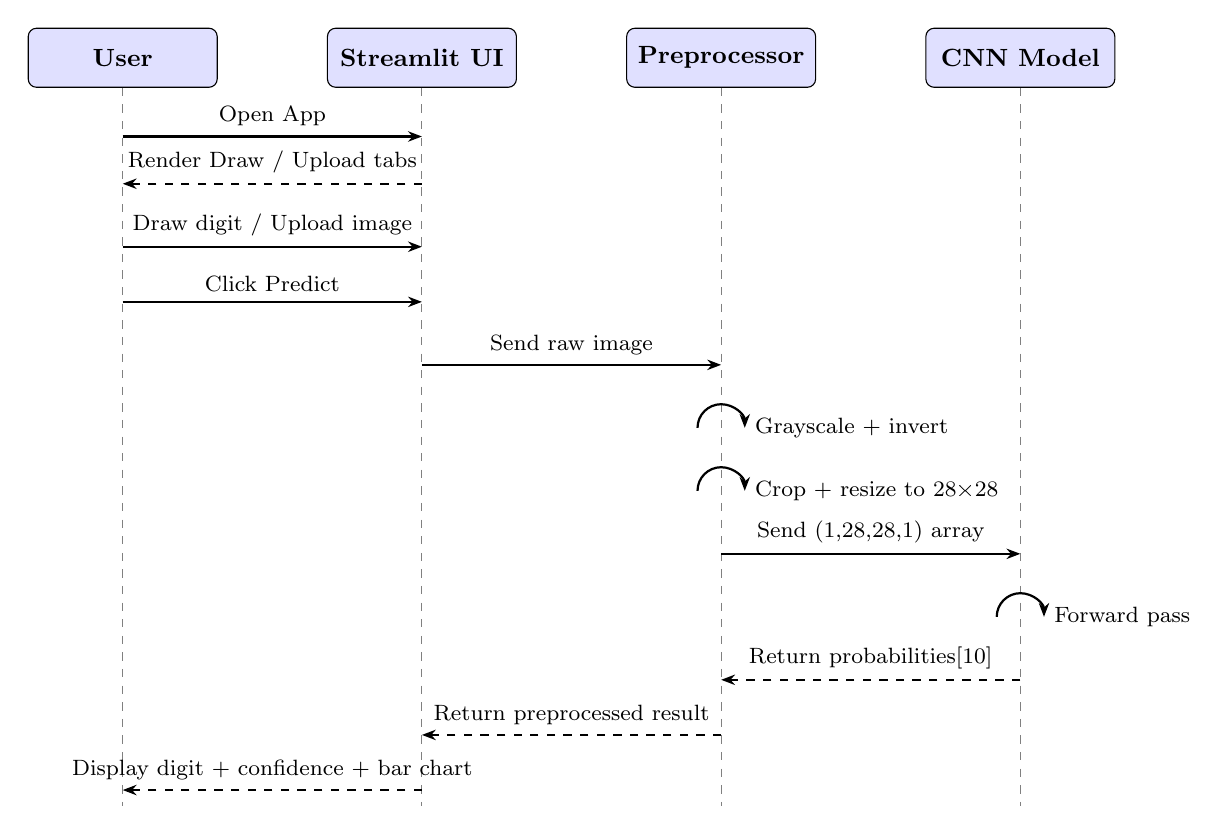
\begin{tikzpicture}[
    lifeline/.style={draw, thick},
    actor/.style={
        draw, rectangle, rounded corners=3pt,
        minimum width=2.4cm, minimum height=0.75cm,
        fill=blue!12, font=\small\bfseries, align=center
    },
    msg/.style={-{Stealth[length=5pt]}, thick},
    ret/.style={-{Stealth[length=5pt]}, thick, dashed},
    note/.style={font=\footnotesize, above, midway}
]

\node[actor] (U)   at (0,   0) {User};
\node[actor] (UI)  at (3.8, 0) {Streamlit UI};
\node[actor] (PP)  at (7.6, 0) {Preprocessor};
\node[actor] (CNN) at (11.4,0) {CNN Model};

\draw[dashed, gray] (U)   -- ++(0,-9.5);
\draw[dashed, gray] (UI)  -- ++(0,-9.5);
\draw[dashed, gray] (PP)  -- ++(0,-9.5);
\draw[dashed, gray] (CNN) -- ++(0,-9.5);

\draw[msg] (0,-1.0) -- (3.8,-1.0)   node[note]{Open App};
\draw[ret] (3.8,-1.6) -- (0,-1.6)   node[note]{Render Draw / Upload tabs};
\draw[msg] (0,-2.4) -- (3.8,-2.4)   node[note]{Draw digit / Upload image};
\draw[msg] (0,-3.1) -- (3.8,-3.1)   node[note]{Click Predict};
\draw[msg] (3.8,-3.9) -- (7.6,-3.9) node[note]{Send raw image};
\draw[msg] (7.3,-4.7) arc(180:0:0.3) node[right, font=\footnotesize]{Grayscale + invert};
\draw[msg] (7.3,-5.5) arc(180:0:0.3) node[right, font=\footnotesize]{Crop + resize to 28×28};
\draw[msg] (7.6,-6.3) -- (11.4,-6.3) node[note]{Send (1,28,28,1) array};
\draw[msg] (11.1,-7.1) arc(180:0:0.3) node[right, font=\footnotesize]{Forward pass};
\draw[ret] (11.4,-7.9) -- (7.6,-7.9) node[note]{Return probabilities[10]};
\draw[ret] (7.6,-8.6) -- (3.8,-8.6)  node[note]{Return preprocessed result};
\draw[ret] (3.8,-9.3) -- (0,-9.3)    node[note]{Display digit + confidence + bar chart};

\end{tikzpicture}
\caption{Sequence Diagram}
\label{fig:sequence}
\end{figure}

\chapter{Experimentation, Results and Discussion}
\section{Experimentation}
During the development of the Handwritten Digit Recognizer, several experiments were carried out to evaluate the performance of the CNN model and the behavior of the application with different types of input. The main aim was to verify that the system correctly identifies digits drawn on the canvas, digits from uploaded images, and handles edge cases gracefully.

\subsection{Model Training Experiment}
The CNN was trained on the MNIST dataset with the following configuration:
\begin{itemize}
    \item Training samples: 60,000 images
    \item Test samples: 10,000 images
    \item Epochs: 10
    \item Batch size: 64
    \item Validation split: 10\% of training data
    \item Optimizer: Adam
    \item Loss function: Sparse Categorical Cross-Entropy
\end{itemize}
The model was monitored for both training accuracy and validation accuracy across all 10 epochs to detect overfitting. The dropout layer (rate 0.5) was effective in keeping the validation accuracy close to the training accuracy.

\subsection{Testing with Drawn Digits}
The first application test was done using the drawable canvas. Digits from 0 to 9 were drawn one by one using the mouse. The system successfully predicted all digits with high confidence when drawn clearly in the center of the canvas. This confirmed that the canvas-to-model pipeline was working correctly.

\subsection{Testing with Uploaded Images}
Next, images of handwritten digits were uploaded to test the preprocessing pipeline. Both dark-on-light (e.g., pencil on white paper) and light-on-dark images were tested. The auto-inversion logic correctly handled both cases by detecting the dominant background color and inverting when necessary. The system produced accurate predictions for clean, single-digit images.

\subsection{Testing with Edge Cases}
Edge cases were also tested to verify robustness:
\begin{itemize}
    \item An empty canvas (no drawing) -- the system displayed a warning message and stopped.
    \item A very small or faint drawing -- the system still attempted a prediction but showed low confidence.
    \item An image with multiple digits -- the system predicted based on the overall content, which may not be accurate for multi-digit inputs.
    \item A non-digit image (e.g., a letter) -- the system returned a prediction with low confidence, indicating uncertainty.
\end{itemize}

\newpage
\section{Results}
After training and testing the Handwritten Digit Recognizer, the system demonstrated strong performance on the MNIST test set and in real-world usage through the application.

\subsection{Model Performance}
The CNN achieved the following results on the MNIST test set after 10 epochs of training:
\begin{itemize}
    \item \textbf{Test Accuracy:} approximately 99\%
    \item \textbf{Test Loss:} approximately 0.03
\end{itemize}
The training and validation accuracy curves showed consistent improvement across epochs with no significant overfitting, confirming that the dropout regularization was effective.

\subsection{Application Performance}
The Streamlit application performed well during all tests:
\begin{itemize}
    \item Predictions were returned instantly after clicking the Predict button
    \item The confidence score and bar chart provided clear and interpretable output
    \item The auto-inversion preprocessing handled both drawn and uploaded images correctly
    \item The application remained stable across multiple consecutive predictions
\end{itemize}

\newpage
\subsection{Screenshots}
\subsubsection{1. Application Home -- Draw Tab}
\begin{figure}[h!]
\centering
\includegraphics[width=0.8\textwidth]{draw_tab.png}
\caption{Draw Tab -- User draws a digit on the canvas}
\end{figure}
This is the main interface of the Handwritten Digit Recognizer showing the Draw tab. The user can draw any digit from 0 to 9 on the black canvas using the mouse or touchscreen. After drawing, the user clicks the Predict button to receive an instant prediction.

\newpage
\subsubsection{2. Prediction Result -- Low Confidence Score}
\begin{figure}[h!]
\centering
\includegraphics[width=0.8\textwidth]{prediction_low.png}
\caption{Prediction Result -- Low Confidence Score}
\end{figure}
This screenshot shows a prediction where the model returns a low confidence score. This typically occurs when the drawn or uploaded digit is ambiguous, poorly centered, or written in an unusual style that differs significantly from the MNIST training data. The bar chart shows probability spread across multiple digit classes, indicating the model is uncertain about the correct digit.

\newpage
\subsubsection{3. Prediction Result -- High Confidence Score (100\%)}
\begin{figure}[h!]
\centering
\includegraphics[width=0.8\textwidth]{prediction_result.png}
\caption{Prediction Result -- High Confidence Score (100\%)}
\end{figure}
This screenshot shows a prediction where the model returns a 100\% confidence score. This occurs when the digit is drawn clearly and closely matches the MNIST training distribution. The bar chart shows the entire probability mass concentrated on a single digit class, with all other classes at or near zero.

\newpage
\subsubsection{4. Upload Tab}
\begin{figure}[h!]
\centering
\includegraphics[width=0.8\textwidth]{upload_tab.png}
\caption{Upload Tab -- User uploads an image of a handwritten digit}
\end{figure}
The Upload tab allows users to upload a photo or scan of a handwritten digit. The system accepts JPG, PNG, BMP, and WEBP formats. A preview of the uploaded image is shown before prediction. The preprocessing pipeline automatically handles both dark-on-light and light-on-dark images.

\newpage
\section{Discussion}
The development and testing of the Handwritten Digit Recognizer demonstrated that a relatively simple CNN architecture is sufficient to achieve near-perfect accuracy on the MNIST benchmark. The two-layer convolutional design with dropout regularization proved effective at learning robust digit representations without overfitting.\\ \\
One important observation during testing was that the preprocessing pipeline plays a critical role in real-world performance. The auto-inversion logic and bounding-box cropping significantly improved the accuracy of predictions on uploaded images, which often differ from the clean MNIST format. Without these steps, the model would struggle with images that have a white background or uncentered digits.\\ \\
The Streamlit framework made it straightforward to deploy the trained model as an interactive application. The drawable canvas component provided a natural way for users to interact with the system, and the confidence bar chart made the model's output interpretable even for non-technical users.\\ \\
However, the system also has limitations. Since the model is trained exclusively on MNIST data, it may struggle with digits written in unusual styles, very thick strokes, or non-standard orientations. The system is also designed for single-digit input only and does not support multi-digit recognition. These are areas that could be addressed in future work.

\chapter{Conclusion and Future Scope}
\section{Conclusion}
The Handwritten Digit Recognizer successfully demonstrates the application of Convolutional Neural Networks for image classification by training a CNN on the MNIST dataset and deploying it as an interactive Streamlit web application. The model achieves approximately 99\% accuracy on the MNIST test set, and the application allows users to draw or upload a digit and receive an instant prediction with a confidence score. The preprocessing pipeline ensures reliable handling of both drawn and uploaded images by automatically adjusting for background color and centering the digit. Overall, the project meets its core objectives and provides a practical, accessible tool that showcases the power of deep learning for handwritten digit recognition.

\section{Future Scope}
The current version of the Handwritten Digit Recognizer focuses on single-digit recognition using the MNIST dataset, but it can be extended in several meaningful ways. Future enhancements may include training on more diverse datasets to improve robustness to different handwriting styles, extending the system to recognize multi-digit numbers or full handwritten words, adding data augmentation during training to improve generalization, deploying the application as a public web service using cloud platforms, integrating a feedback mechanism where users can correct wrong predictions to continuously improve the model, and exploring more advanced architectures such as ResNet or EfficientNet for even higher accuracy.

\newpage
\section*{References}

\begin{enumerate}[label={[{\arabic*}]}]
    \item Y. LeCun, L. Bottou, Y. Bengio, and P. Haffner, "Gradient-Based Learning Applied to Document Recognition," \textit{Proceedings of the IEEE}, vol. 86, no. 11, pp. 2278--2324, 1998.
    \item N. Srivastava, G. Hinton, A. Krizhevsky, I. Sutskever, and R. Salakhutdinov, "Dropout: A Simple Way to Prevent Neural Networks from Overfitting," \textit{Journal of Machine Learning Research}, vol. 15, pp. 1929--1958, 2014.
    \item A. Krizhevsky, I. Sutskever, and G. Hinton, "ImageNet Classification with Deep Convolutional Neural Networks," \textit{Advances in Neural Information Processing Systems}, vol. 25, 2012.
    \item K. O'Shea and R. Nash, "An Introduction to Convolutional Neural Networks," \textit{arXiv preprint arXiv:1511.08458}, 2015.
    \item TensorFlow Documentation, \textit{https://www.tensorflow.org/api\_docs}
    \item Streamlit Documentation, \textit{https://docs.streamlit.io}
    \item I. Goodfellow, Y. Bengio, and A. Courville, \textit{Deep Learning}. Cambridge, MA: MIT Press, 2016.
    \item D. P. Kingma and J. Ba, "Adam: A Method for Stochastic Optimization," \textit{arXiv preprint arXiv:1412.6980}, 2014.
    \item L. Deng, "The MNIST Database of Handwritten Digit Images for Machine Learning Research," \textit{IEEE Signal Processing Magazine}, vol. 29, no. 6, pp. 141--142, 2012.
    \item V. Nair and G. E. Hinton, "Rectified Linear Units Improve Restricted Boltzmann Machines," in \textit{Proceedings of the 27th International Conference on Machine Learning (ICML)}, pp. 807--814, 2010.
    \item S. Ioffe and C. Szegedy, "Batch Normalization: Accelerating Deep Network Training by Reducing Internal Covariate Shift," in \textit{Proceedings of the 32nd International Conference on Machine Learning (ICML)}, pp. 448--456, 2015.
    \item NumPy Documentation, \textit{https://numpy.org/doc}
    \item Pillow (PIL) Documentation, \textit{https://pillow.readthedocs.io}
\end{enumerate}

\end{document}
